\documentclass{article}

\usepackage{amsmath, amssymb}
\usepackage{graphicx}
\usepackage[margin=0.5in]{geometry}

\graphicspath{{images/}}

\DeclareMathOperator*{\argmin}{arg\,min}
\DeclareMathOperator*{\argmax}{arg\,max}

\begin{document}

\title{Memory Networks}
\author{Piyush Patil}
\maketitle

Although neural networks can, in principle, learn any function, in practice the network topology required is often infeasible to implement and requires too much labelled data. In particular, when it comes to heavily context dependent tasks, such as dialogue, neural nets perform sub-optimally because the way they "store" memory is too distributed, tangled, and doesn't scale well with the network topology. The addition of some long-term memory component to the network might solve some of these issues, providing a compartmentalized, long-term, and potentially very large bank in which to store data - the key is to get the network to learn on its own how to read and write to the memory. \textit{Memory networks} are a general term for neural models augmented with some kind of long-term memory bank.

\section{Architecture}
\textbf{(Definition) Memory network}: \textit{A \textbf{memory network} is a set of four components $ I, G, O, R $ equipped with a \textbf{memory} $ m $. We define the components as follows.}
\begin{enumerate}
    \item $ I $ is the \textbf{input feature map}, and is a function converting incoming input to their internal feature representation.
    \item $ G $ is the \textbf{generalization module}, and accepts input which is used to update the memory. This gives the whole model a chance to compress and generalize the stored memories once it's seen new input.
    \item $ O $ is the \textbf{output feature map}, a function using input feature vectors and the memory to output a feature vector.
    \item $ R $ is the \textbf{response module} and simply converts the output feature vector into the appropriate object.
\end{enumerate}
\indent \textit{The memory $ m $ is simply a vector of objects.}
Memory networks thus define a pipeline in which raw incoming data is first transformed to a feature representation the model can use, which is then used to update the memory bank, followed by the transformation of the input into an output in a way that relies on the memory, followed by a conversion of the output featurization back to the native space the input was in. Ideally all of these components would be able to be trained in supervised learning.
\newline
More formally, given input $ x $ (this could be any kind of raw data, such as a string of characters, an audio signal, etc.), the model first converts the input to a feature representation, $ I(x) $. The memory $ m $ is then updated with
$$ \forall i: m_i = G(m_i, I(x), m) $$
Following the memory update, the output mapping uses the input feature vector and memory to produce an output:
$$ o = O(I(x), m) $$
The output is then decoded to the form we want, $ r = R(o) $, which is the response of the model. The structure is intentionally very general, and the components $ I, G, O, $ and $ R $ can be any vanilla machine learning model, such as an SVM, decision tree, or feedforward neural net. Notice that no differentiability or even continuity requirement is placed on the components, so the model need not be end-to-end trainable with gradient descent.

\section{End to End Memory Networks}
The above architecture is sufficiently general so as to allow for models which require modular training - each model must be trained independently and then connected together, rather than in one end-to-end training phase. However, models which are completely differentiable, from input to output, can be trained easily in one phase, end-to-end, allowing the modules to be trained jointly, often yielding better performance. Let's look at one specific example of such an end-to-end memory network, whose architecture consists of a neural network with a recurrent attention model over a (possibly very large) external memory.
\newline
The model we'll present is an RNN architecture in which the recurrence reads from an external memory several times before outputting anything; the reading and writing operations are continuous implementations of the general $ O $ and $ G $ modules outlined above. The end-to-end continuity allows us to train the model with backpropagation using only input-output pairs, reducing the training to a simple supervised learning task. The model is designed for language modeling, and the approach we'll take is as follows.
\newline
For input, the model will take a set of symbols $ x_1, \cdots, x_n $ as well as a symbolic query $ q $. It'll output an answer $ a $, which is also a symbol. By symbol we mean that each of the $ x_i $, $ q $, and $ a $ come from a dictionary $ V $ of words. We're using the term "symbol" here as a more general term than "word", but the primary focus of this model is still NLP. The way we've set up the inputs to this problem is conducive to learning NLP tasks, such as conversational or dialogue-based NLP, which consists of taking the full conversation up to the present (ie the $ x_i $) and the last heard utterance (ie $ q $), and producing a response (ie $ a $). The model will first take the $ x_i $ and write them to memory, and then try to find a continuous representation of the $ x_i $ and $ q $. This continuous representation is then processed with multiple \textit{memory hops}, producing the output symbol $ a $. Let's look at the single-layer case of the model, which implements a single memory hop operation, and then generalize to the full model by showing how single memory hops can be stacked on top of each other. Before we look at the single-layer case, we'll take a brief aside to look at word embeddings, which will form the input feature map.

\subsection{Word Embeddings}
To use a neural network to operate on abstract symbols, we'll first need to embed the symbols in some vector space, to enable us to do all the operations required by a neural net. In particular, since words symbols are initially represented as one-hot vectors, we need an \textit{embedding map}, mapping symbols from their extremely high-dimensional ($ | V | $-dimensional to be precise) and sparse space onto a lower-dimensional, dense, continuous vector space, such as a manifold; we want the embedding map to be continuous, not only to ensure the end-to-end trainability of the model, but also because we'd like similar or "near by" symbols to be embedded in similar locations in the vector space. The entire idea behind word embeddings is based on the \textit{distributional hypothesis}, that words that share context or have similar distributions (such as probability distributions learned by a language model) throughout a dataset are semantically similar.
\newline \newline
The question remains of how to find a good embedding map. If the dictionary $ V $ is finite, then we could always use one-hot vectors to encode symbols, and this would, in theory, have the same representing power as any other word embedding. However, a strong embedding which maps synonymous words close to each other and otherwise is able to quantitatively model linguistic relationships well in high-dimensional space will be provide for a much easier learning task for any machine learning model. To find a good embedding, we can actually use machine learning to train a good word embedding. This would essentially involve taking some parameterized function as our word embedding and initializing it randomly, and then using a large number of examples of text that is grammatically sound and logically consistent, as well as examples that aren't. To make this a full supervised learning task, we also would need to introduce some discriminator module which runs on top of the word embedding and predicts, for example, if a given $ n $-gram or sentence is linguistically valid or not. We could train such a system with gradient descent, and be left with a word embedding that had been forced to learn a good way of representing words in such a way as to allow the discriminator module to accurately classify sentences as valid or not. Common labels include taking valid sentences and turning them into invalid ones by randomly changing some of the words to other words, or simply by getting the system to take an incomplete sentence and predict the next word.

\subsubsection{Neural Word Embeddings}
First, let's go over the background behind how to use neural techniques (as opposed to ones based on the statistics of the dataset, such as analyzing the co-occurrence marix) to learn a word embedding. Recall that a \textit{language model} is a probability distribution on the words of a dataset, and aims to learn a function for predicting the probability that a target word appears conditioned on certain context words. For instance, a good language model would probably compute
$$ \Pr(\text{"mat" } | \text{ "the cat sits on the"}) $$
to be fairly high. More generally, neural language models are trained with maximum likelihood, and as such try to maximize
$$ \Pr(w_t | h) = \text{softmax}(s(w_t, h)) = \frac{e^{s(w_t, h)}}{\sum_{w \in V} e^{s(w, h)}} $$
where $ w_t $ is the target word and $ h $ is the history, containing the last several context words, and $ s $ is some scoring function representing the compatibility of $ w_t $ with the history. The log-likelihood, then, is
$$ \log \left( \Pr(w_t | h) \right) = s(w_t, h) - \log \left( \sum_{w \in V} e^{s(w, h)} \right) $$
We need to learn a scoring function which maximizes the above. Although this can be done easily by choosing a differentiable scoring function, parameterizing it, and using gradient ascent on the log-likelihood to find a maximum with respect to the parameters. In practice, this is very computationally taxing, since we have to iterate through our entire dictionary at every training step.

\subsubsection{Word2Vec}
 Let's look at one of the most common embeddings used in practice - word2vec. If we use word2vec, however, we can take a much more feasible approach. The key is that we don't need a full probabilistic model; instead, the approach we take is to train a binary classifier - specifically, using logistic regression - to, given the history of context words $ h $, distinguish between the real target words that fit the history and $ k $ noise words in the same context. The idea here is that the appropriate target word doesn't need to be compared against every other word in the dataset to find the probability. Rather, we only need to compare against the other $ k $ words in the context, since those are the most likely to throw off the probability. Mathematically, our objective function here is
 $$ J = \log(Q_\theta (D = 1 | w_t, h)) + k \mathbb{E}[ \log(Q_\theta (D = 0 | v, h)) ] $$
 where $ v $ is a random variable whose range is the $ k $ noise words, with some assumed underlying probability distribution $ P_{\text{noise}} $. $ Q $ is the logistic regression probability that a given word and history came from the dataset $ D $, which is a way of saying the probability that we'd observe the given word-history combination in the dataset. $ \theta $ is a set of learned embedding vectors which parameterize $ Q $; our goal is to maximize the objective function, and this happens precisely when the model learns to assign high probabilities to real target words and low ones to noise words.
\newline \newline
To recap, we train a word2vec embedding on a corpus of text by first creating our dataset $ D $ which takes the text and produces a set of context-word pairs for each word in the text. The precise definition of \textit{context} can depend on the task, but the most common way of defining it is with a "window of words" - the context of a word is simply the sequence of the surrounding (ie to the left and to the right) $ 2 m $ words, where $ 2 m + 1 $ is the window size. We then take the above objective function and optimize it with stochastic gradient descent. We also don't compute the expectation analytically, instead approximating it with sampling.
\newline \newline
The simplest embedding map is to simply use an embedding matrix $ A \in \mathbb{R}^{d \times | V |} $, where $ d $ is the dimension of the vector space we're embedding in, and therefore also the dimension of the memory vectors stored in the memory matrix $ M \in \mathbb{R}^{d \times N} $. All this means is that we define our embedding function to act on a symbol (ie a word) by first mapping it to its one-hot vector representation, and then multiplying it by $ A $. In other words, our embedding map is simply a linear transformation, parameterized by the matrix $ A $.

\subsubsection{Continuous Sentence Representations}
Although the initial specification of the model involves a set of symbols $ x_i $ and a query symbol $ q $, the motivating application of this model involves the symbols being \textit{sentences}, not words. This means that we need to find a way to embed sentences in a continuous vector space, rather than words as described above. This problem is an active area of research in its own right, and there has been some success in applying variational autoencoders and LSTM RNNs to the task, but here we offer two much simpler options, which simply build off of traditional word embeddings.
\newline \newline
Given an embedding matrix $ A $, let $ s_i = (x_1, \cdots, x_n) $ be a sentence of symbols from the dictionary $ V $. The first sentence representation we look at is a rather weak one - \textit{continuous bag-of-words}. In this scheme we simply add the embeddings of each word together:
$$ m = \text{ sentence embedding of $ s_i $ } = \sum_{j = 1}^n A x_j $$
This simplistic model has the glaring flaw that it throws away all context and ordering of the words, which are obviously critical to the sentence's meaning. We can modify this approach to be context-dependent by adding a weighting factor in the sum which forces the embedding to account for a word's position:
$$ m = \sum_{j = 1}^n l_j \cdot A x_j $$
where $ l_j $ is the column vector defined by
$$ (l_j)_k = \left( 1 - \frac{j}{n} \right) - \frac{k}{N} \cdot \left( 1 - \frac{2 j}{J} \right) $$
where $ N $ is the total number of sentences.

\subsection{Single Layer Case}
Let's now look at the single-layer case of the model. We can take the $ x_i $ and $ q $ and embed them, maybe with some embedding matrix $ A $, in a continuous space. In this way, we can map each $ x_i $ to an $ m_i $, which we'll view as a memory vector that we will soon write to the memory matrix $ M $. Similarly, we'll map $ q $ to some internal representation of the query, $ u $ using another embedding matrix, $ B $. Now that we're in our embedding space, we can now iterate over every memory vector $ m_i $ in the memory matrix and compute its similarity with the query $ u $, to find the closest symbol in our memory to the query. The simplest way to do this is using cosine distance, followed by a softmax transformation:
$$ p = \text{softmax}(u^\intercal M) $$
This gives us a probability vector $ p $ over our inputs, which is dependent on how similar $ q $ is to each of the $ x_i $. This is useful because what we're doing here is searching the conversation up to the present for relevant information to the query. Our output will simply be the "average" of the conversation so far, in the sense of taking the sum of each of the $ x_i $ weighted by their probability $ p_i $. Of course, we can't actually add up the $ x_i $, so we'll need another embedding determined by some embedding matrix $ C $ (we don't reuse the embedding matrix $ A $ here since the former was presumably trained with the goal of storing words in memory, whereas right now we want to map each $ x_i $ to some output vector, a different task). This associates each $ x_i $ with an output vector $ c_i $, and we can now define out output to be
$$ o = \sum_{i = 1}^n p_i c_i $$
where $ p_i $ is the $ i^{\text{th}} $ entry of the probability vector $ p $. We can use the \textit{response vector} $ o $ above to generate the final response $ a $ by taking the sum of our embedded query $ u $ and the response vector, and passing through a weight matrix, followed by a softmax normalization:
$$ a = \text{softmax}(W \cdot (o + u)) $$
The reason we apply the softmax normalization is to convert our final output vector (ie $ W \cdot (o + u) $) to a probability distribution for which symbol from the dictionary the model is outputting. This is exactly what we'd want in our loss function, when we compare $ a $ to the correct symbol, represented as a one-hot representation. The following diagram depicts the full model in this simple case.

\begin{center}
    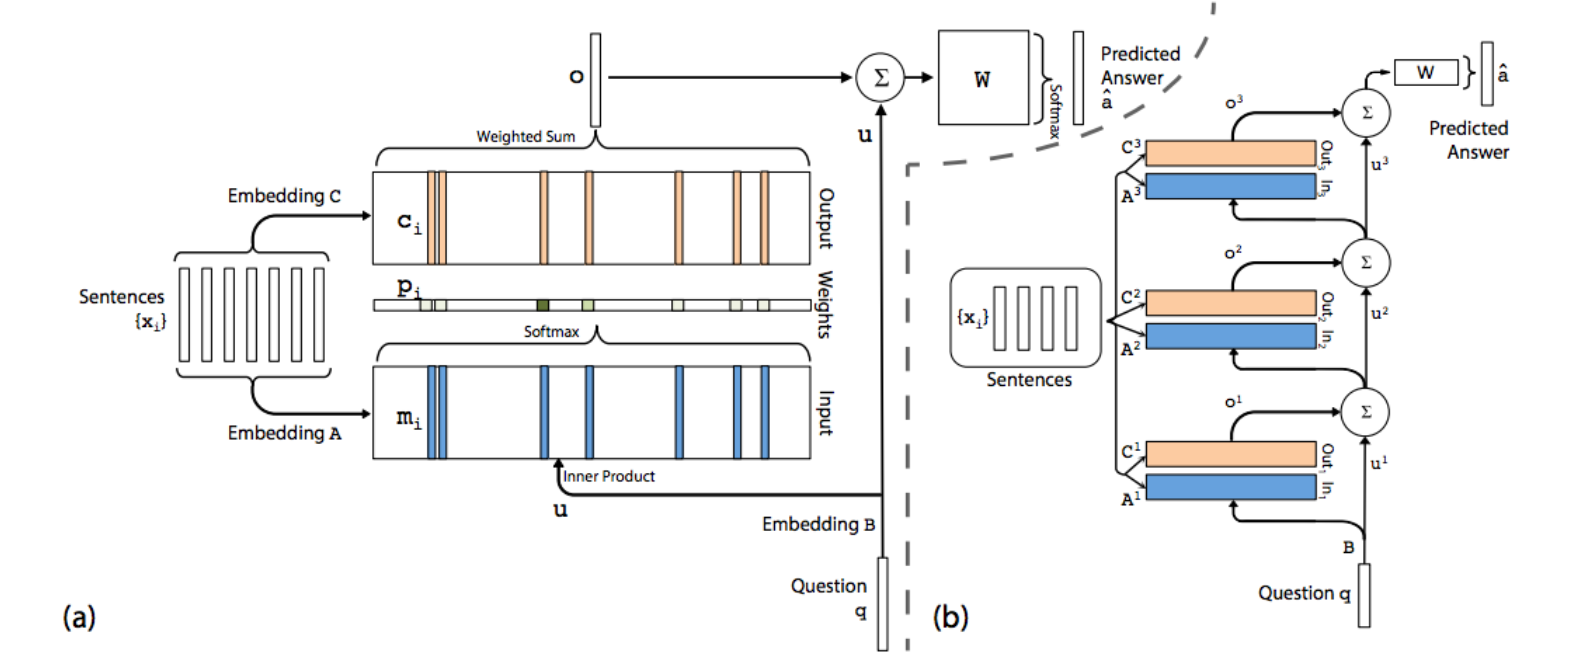
\includegraphics[scale=0.5]{images/endtoendsinglelayer.png}
\end{center}

On the left is the single layer case, and on the right is an example with three layers.

\subsection{Multiple Layer Case}
Let's now extend the single layer case to $ L $ layers by stacking the above memory hops. We can perform the stacking as follows. Each layer $ l $ has its own embedding matrices $ A^l $ and $ C^l $ for the input conversation. 
\newline
In the single layer case, $ u $, the embedded form of the query, was the input to the layer, along with the memory. The output of the layer was the sum of the response vector and the input $ u $. To generalize this, we can construct layer $ l $ as follows. As with any neural network, layer $ l $ takes as input the output of the previous layer, call it $ u^l $, as well as the memory $ M $. The layer then produces a response vector $ o^l $ just the same as in the single layer case, except using $ u^l $ as the "embedded query" instead of $ u^1 = u = B q $:
$$ M^l = \begin{bmatrix} m_i \end{bmatrix}_{1 \leq i \leq n} \text{ where } m_i = A^l x_i $$
$$ p^l = \text{softmax} \left( (u^l)^\intercal M^l \right) $$
$$ c^l_i = C^l x_i $$
$$ o^l = \sum_{i = 1}^n p^l_i c^l_i $$
Just as in the single layer case, the output of the vector is the sum of the "embedded query", in this case $ u^l $, and the response vector $ o^l $:
$$ u^{l + 1} = u^l + o^l $$
Of course, since we're merely stacking layers here we don't pass through a softmax normalizer, and we also don't use any weights. Layer $ l + 1 $ repeats the process, taking $ u^{l + 1} $ as input. At the very last layer, we re-introduce the weight matrix and as usual pass through a softmax function, so the final output of the full model is
$$ a = \text{softmax}(W \cdot (u^L + o^L)) $$

\subsubsection{Weight Tying}
This model is reminiscent of a recurrent neural network, since each layer takes as input not only the output of the last layer but also a novel embedding of the same shared memory matrix of context. Inspired by this connection, it's common to reduce the dimensionality of the parameter space by using RNN-like weight sharing. In particular, the following are two possible weight tying schemes.
\newline
\begin{enumerate}
    \item \textbf{Adjacent Weight Tying}: In this scheme, the output embedding of a layer becomes the input (or memory) embedding of the next layer, ie
        $$ \forall l \in \{ 1, \cdots, L \}: C^l = A^{l + 1} $$
    The motivation for this is that when we extend a single-layer memory network by stacking memory hops, the idea behind doing so is that the output of one intermediate memory hop serves as some intermediate sentence representation of a combination of the query with the context, which is intended to learn dependencies and project to a manifold that allows the subsequent layer to more easily learn its own features about the text; as such, it makes sense then to re-use the way we embedded the sentence representation for one layer when we embed the query and context in the next layer.
    \newline
    We impose the following additional constraints: rather than adding another answer prediction weight matrix, we simply use the last output embedding matrix.
        $$ W = C^L $$
    Moreover, the initial query embedding is the same as the initial memory embedding
        $$ B = A^1 $$
    \item \textbf{Layer-wise}: This scheme is more closely inspired by the structure of an RNN. Here we do use separate input and output embeddings, but constrain them to be the same across all layers.
        $$ A^1 = \cdots = A^L \text{ and } C^1 = \cdots = C^L $$
    This is directly inspired by the shared weights of an RNN, and increases the similarity between each memory hop and an RNN layer. Sometimes a linear mapping $ H $ is added to the update equation for each memory hop. This linear mapping is a parameter that's learned during training, and experimentally has been shown to increase accuracy.
        $$ \forall l \in \{ 1, \cdots, L \}: u^{l + 1} = H u^l + o^l $$
\end{enumerate}

\end{document}
